\documentclass[landscape]{jhuslides3C}
\usepackage{url}
\usepackage{amsmath}
\usepackage{graphicx}
\usepackage{color}
\usepackage{colortbl}
%\usepackage{epic,ecltree}
%\usepackage{bar}
%\usepackage{qtree}
%\usepackage{eclbip}
\usepackage{fancybox}
\usepackage{pause} % java -jar ~/Code/bin/pp4p.jar mtsummit09-talk.pdf mtsummit09-talk.view.pdf
\usepackage[absolute]{textpos}
\pdfoptionpdfminorversion 3
%\usepackage{courier}
\usepackage{tikz}
%\usepackage{tikz-qtree}
\usetikzlibrary{calc,matrix}
%\usepackage{algorithmic}
%\usepackage{algorithm}
\usepackage{amssymb,latexsym} % for \blacklozenge
%\renewcommand{\algorithmicrequire}{\textbf{Input:}}
%\renewcommand{\algorithmicensure}{\textbf{Output:}}
%\renewcommand{\algorithmiccomment}[1]{// {\em #1}}
\usepackage{multicol}
\usepackage{wasysym} % smileys
%\usepackage{lmodern}
%\ttfamily
\usepackage{palatino}
\renewcommand*\ttdefault{txtt} % 20% tighter than courier
%\usepackage[T1]{fontenc}

\usepackage{hyperref}

\definecolor{lightblue}{rgb}{.8,.8,1}
\definecolor{mediumlightblue}{rgb}{.5,.5,1}
\definecolor{lightyellow}{rgb}{1,1,.5}
\definecolor{lightorange}{rgb}{1,.9,.7}
\definecolor{darkorange}{rgb}{1,.75,.2}
\definecolor{sortadarkorange}{rgb}{.8,.5,.1}
\definecolor{verydarkorange}{rgb}{.5,.3,0}
\definecolor{darkblue}{rgb}{0,0,0.8}
\definecolor{verydarkgreen}{rgb}{0,0.4,0}
\definecolor{darkgreen}{rgb}{0,0.8,0}
\definecolor{darkred}{rgb}{0.8,0,0}
\definecolor{verydarkred}{rgb}{0.6,0,0}
\definecolor{lightgreen}{rgb}{.8,1,.8}
\definecolor{lightred}{rgb}{1,.8,.8}
\definecolor{darkgrey}{rgb}{0.5,0.5,0.5}
\definecolor{purple}{rgb}{0.6,0,0.6}
\definecolor{red}{rgb}{1,0,0}
\definecolor{orange}{rgb}{.8,.6,0}
\definecolor{cyan}{rgb}{0,.6,.6}
\definecolor{reddishgreen}{rgb}{0.4,0.6,0}

\newcommand{\newconcept}[1]{\textcolor{blue}\textbf{#1}}
\newcommand{\example}[1]{\textcolor{darkblue}{\rm #1}}
\newcommand{\important}[1]{\textcolor{darkblue}{\em #1}}
\newcommand{\concept}[1]{\textcolor{darkblue}{\em #1}}
\newcommand{\maths}[1]{\textcolor{purple}{#1}}
\newcommand{\mathstt}[1]{\textcolor{purple}{$\mathtt{#1}$}}
\newcommand{\reference}[1]{\vspace{-2mm}\begin{flushright}\textcolor{purple}{\tiny [from #1]}\end{flushright}\vspace{-7mm}}
\renewcommand{\url}[1]{\textcolor{verydarkred}{\tt #1}}

\newcommand{\highlightbox}[6]{\begin{textblock}{#3}(#1,#2) \colorbox{#4}{\textcolor{#5}{\begin{minipage}{#3in} #6 \end{minipage} }} \end{textblock}}
\newcommand{\backgroundbox}[5]{\highlightbox{#1}{#2}{#3}{#5}{black}{\vspace{#4in}\hspace{#3in}}}
\newcommand{\currenttopic}[1]{\colorbox{lightyellow}{\textcolor{black}\textbf{#1}}}

\newcommand{\littlecode}[1]{\colorbox{gray}{\textcolor{black}{\small \tt #1}}}
\newcommand{\highlight}[1]{\colorbox{lightyellow}{#1}}
\newcommand{\highlightOrange}[1]{\colorbox{lightorange}{#1}}
\newcommand{\highlightGreen}[1]{\colorbox{lightgreen}{#1}}
\newcommand{\highlightBlue}[1]{\colorbox{lightblue}{#1}}


%%%%%%%%%%%%%%%%%%%%%%%%%%%%%%%%%%%%%%%%%%%%%%%%%%%%%%%%%%%%%%%%%%%%%%%%%%%%

\begin{document}\rm
\title[Introduction to Human Language Technology: Information Extraction]{Information Extraction}
\author[Philipp Koehn]{Philipp Koehn}
\date{28 October 2019}
\maketitle

%%%%%%%%%%%%%%%%%%%%%%%%%%%%%%%%%%%%%%%%%%%%%%%%%%%%%%%%%%%%%%%%%%%%%%%%%%%%

\slide{Text $\rightarrow$ Knowledge}
\vfill
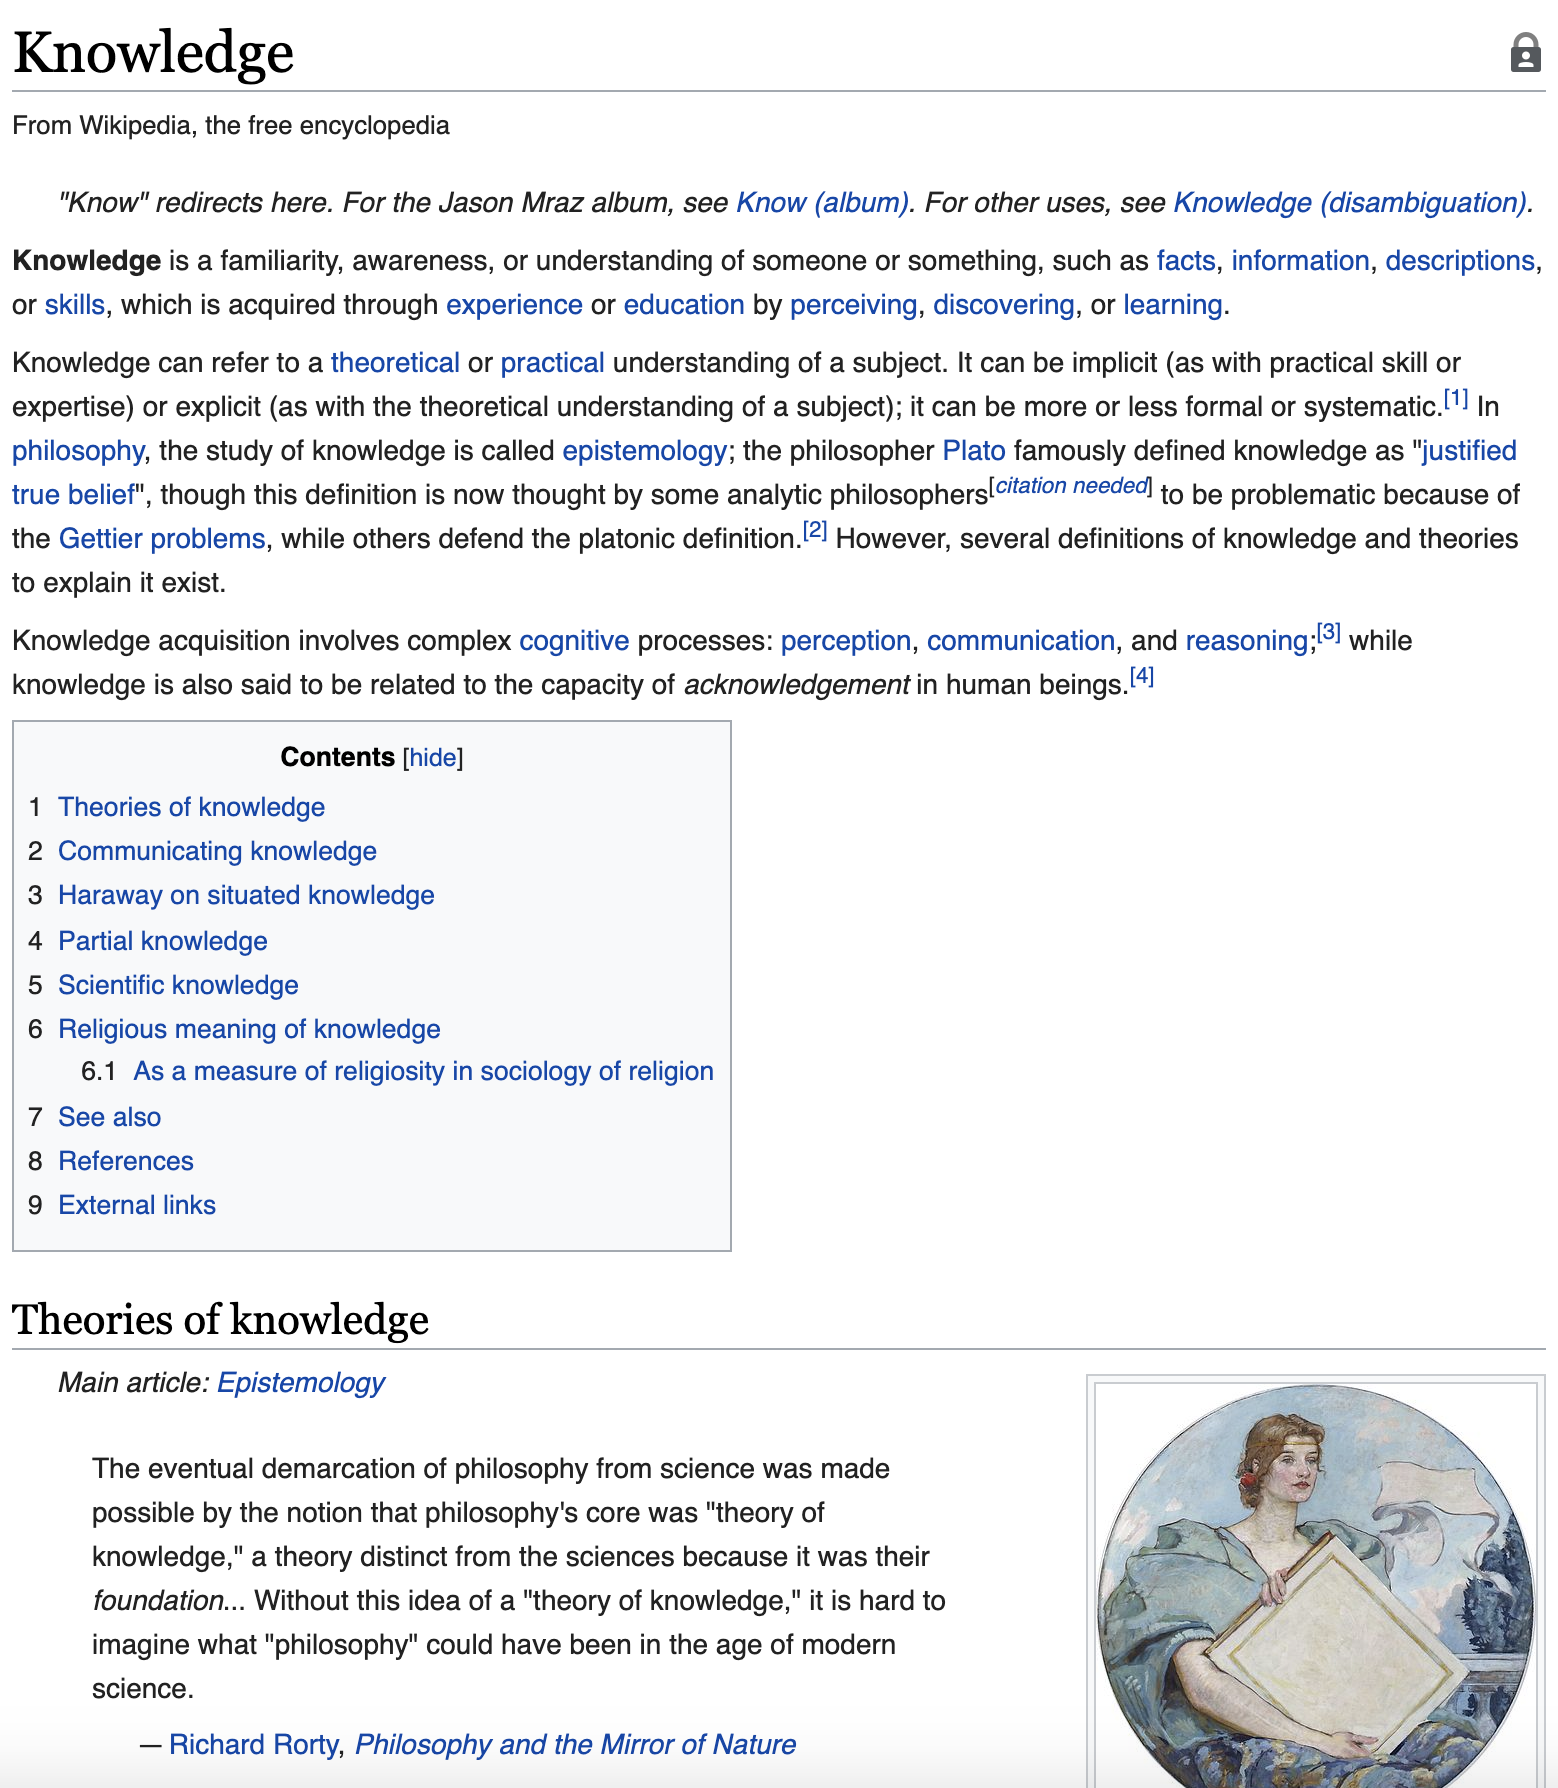
\includegraphics[scale=0.35]{wikipedia-knowledge.png}
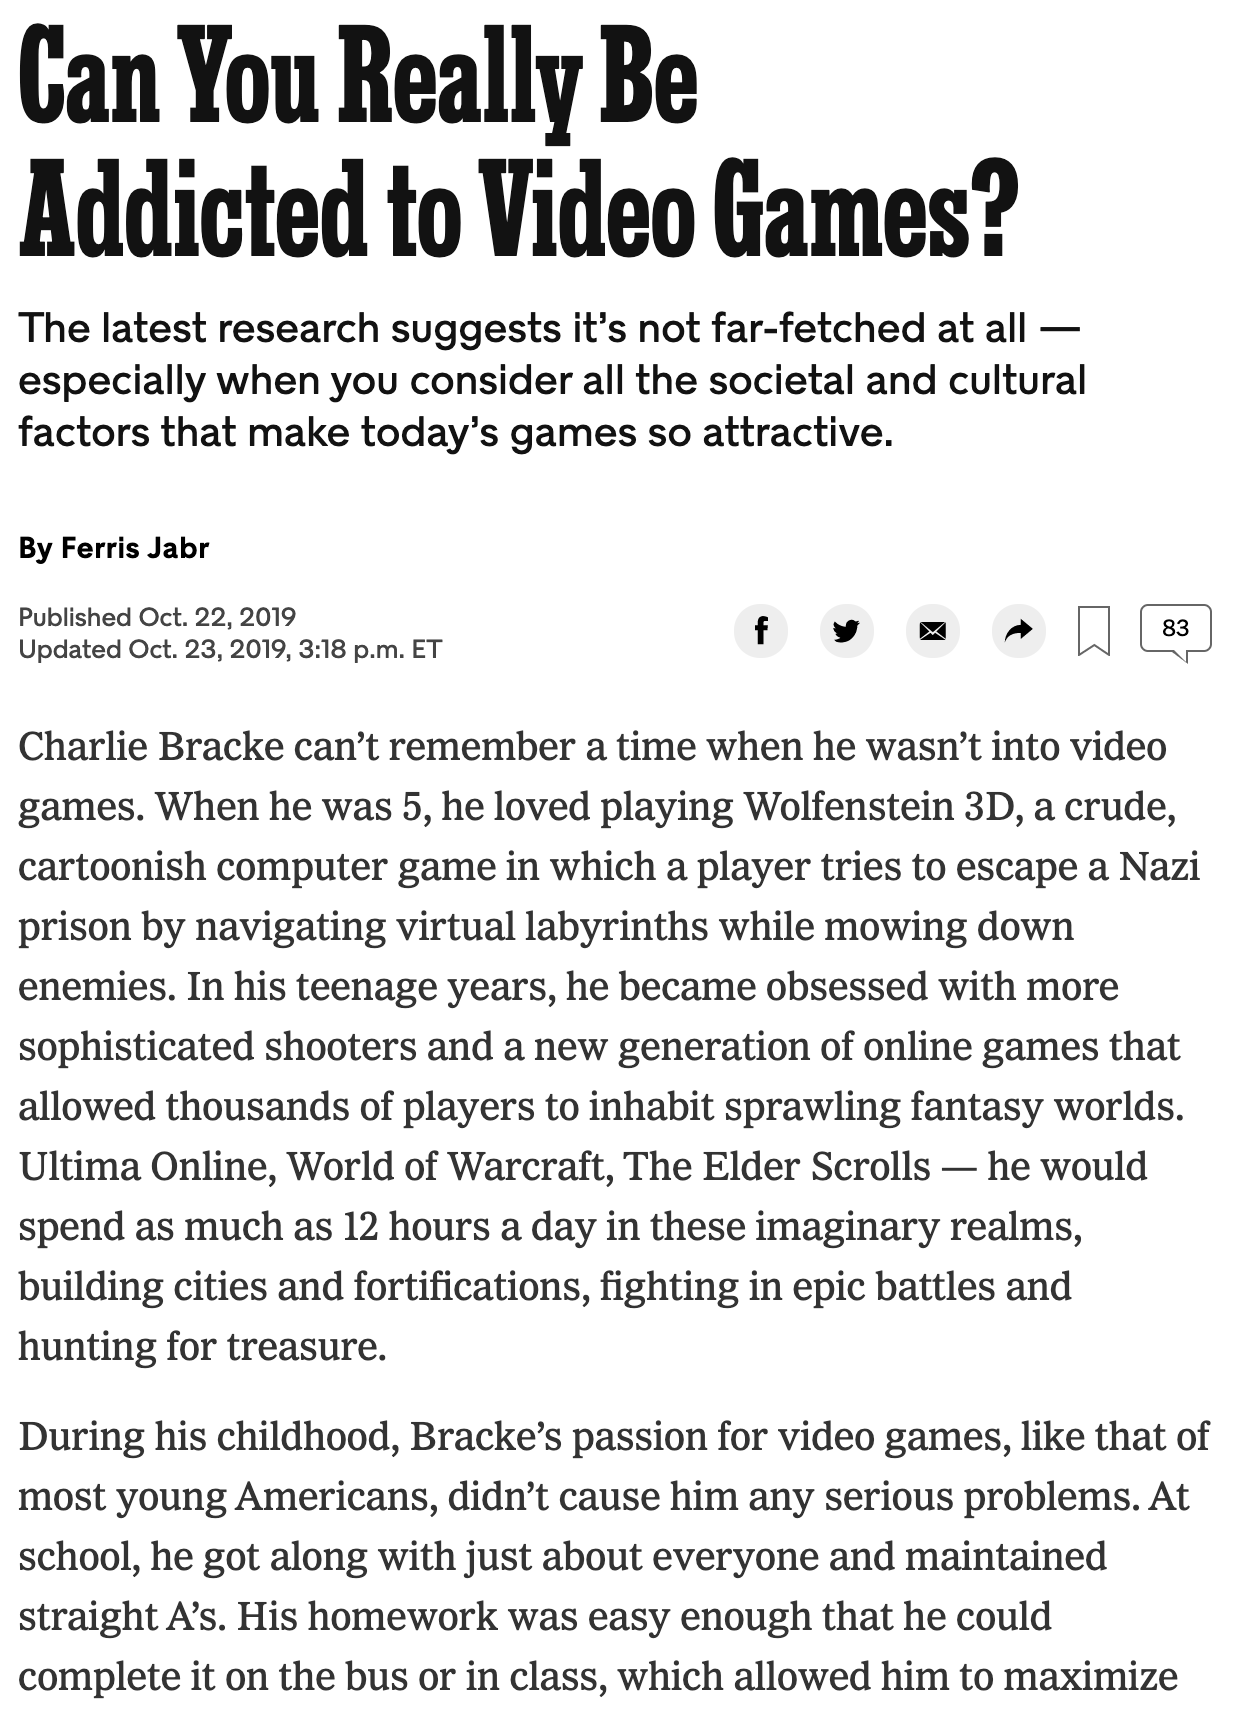
\includegraphics[scale=0.35]{nytimes-article.png}
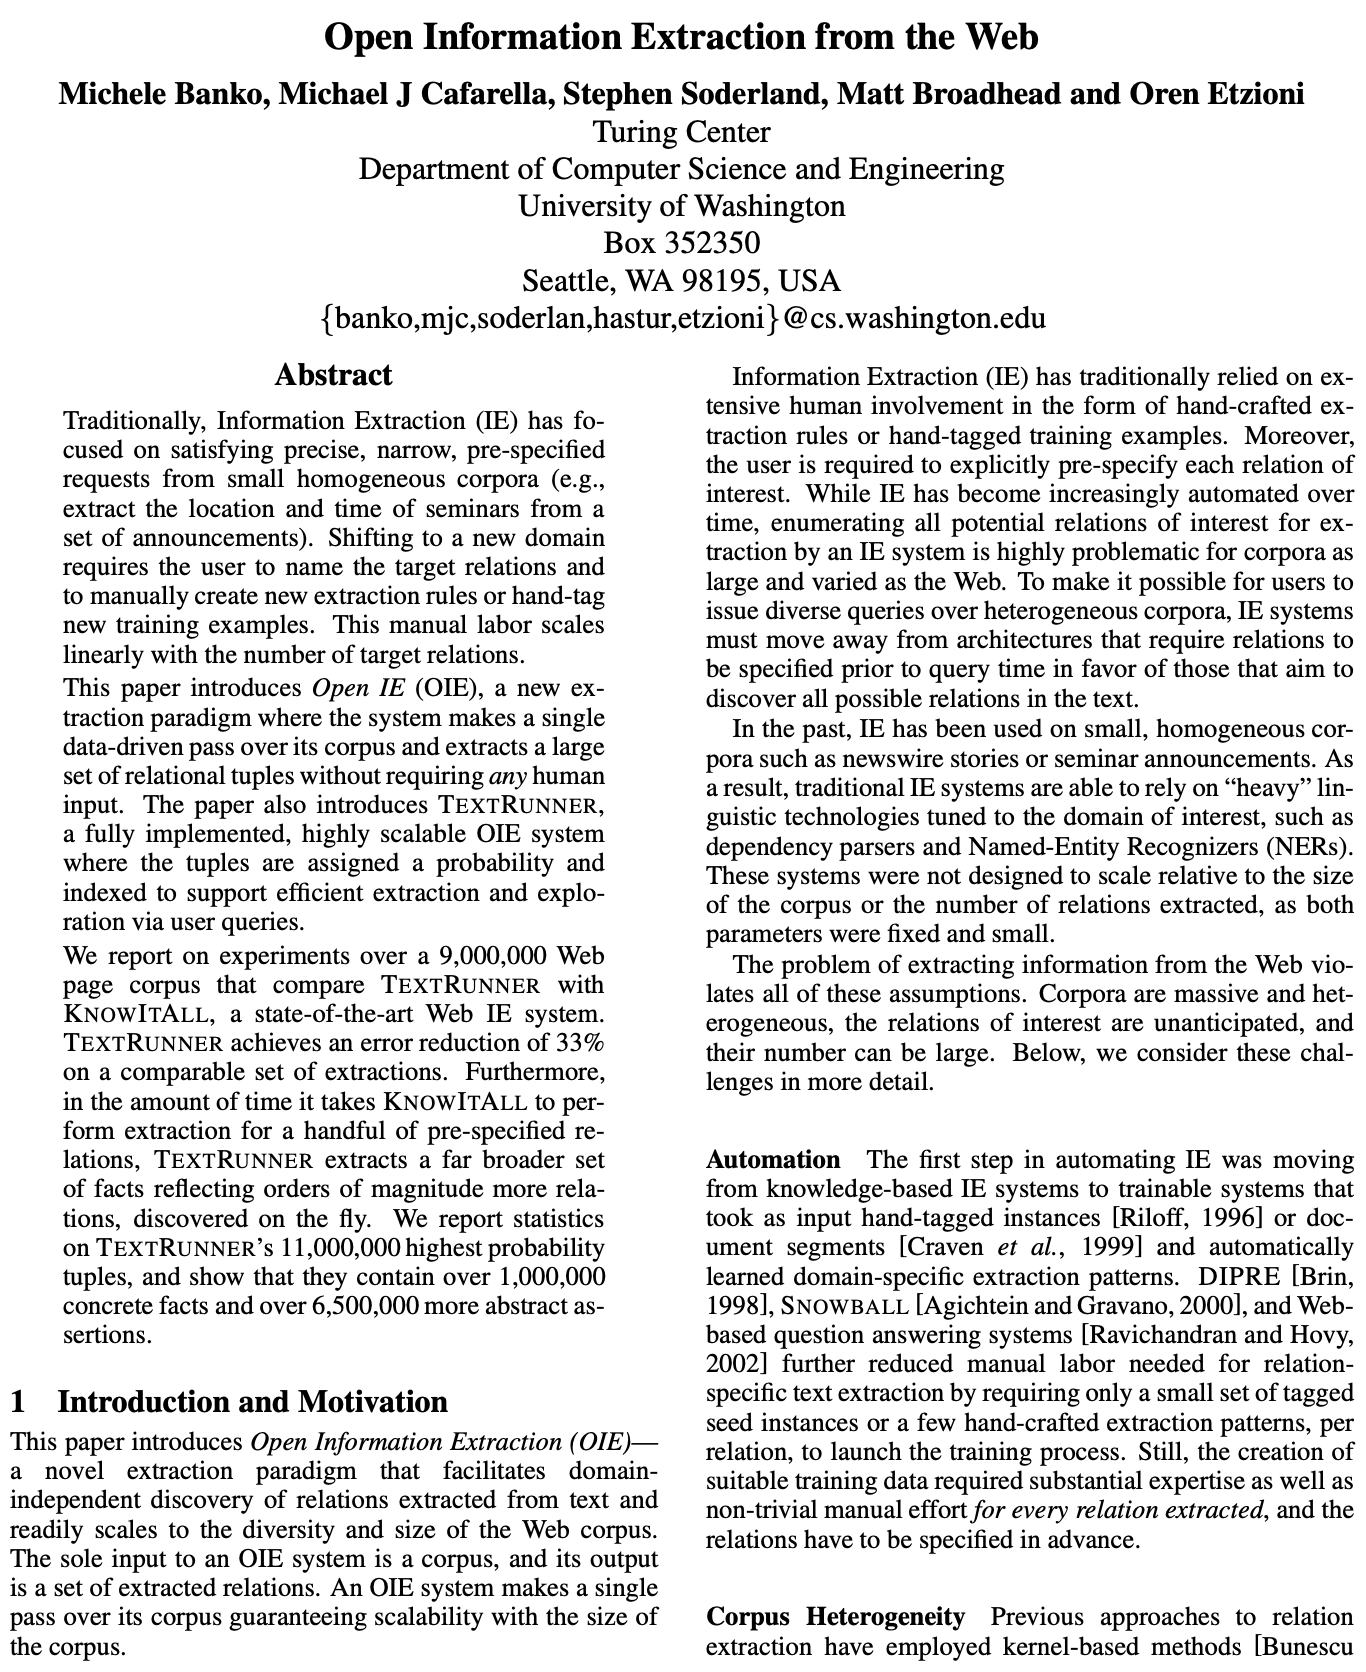
\includegraphics[scale=0.35]{research-paper-ie.png}
\begin{itemize}\itemsep 0mm
\item Human knowledge is stored in text
\item How can we extract this to make it available for processing by machines?
\end{itemize}
\vfill

%%%%%%%%%%%%%%%%%%%%%%%%%%%%%%%%%%%%%%%%%%%%%%%%%%%%%%%%%%%%%%%%%%%%%%%%%%%%

\slide{}
\vspace{85mm}
\begin{center}
{\huge examples}
\end{center}

%%%%%%%%%%%%%%%%%%%%%%%%%%%%%%%%%%%%%%%%%%%%%%%%%%%%%%%%%%%%%%%%%%%%%%%%%%%%

\slide{Goal: Build Database of World Leaders}
\vfill
\begin{tabular}{|c|c|c|}\hline
\bf Country & \bf Position & \bf Person\\ \hline \hline
United States & president & George Walker Bush \\ \hline
United States & president & Barack Hussein Obama \\ \hline
United States & president & Donald Trump\\ \hline
Germany & chancellor & Gerhard Schr\"oder \\ \hline
Germany & chancellor & Angela Merkel \\ \hline
United Kingdom & prime minister & Theresa May \\ \hline
United Kingdom & prime minister & Alexander Boris de Pfeffel Johnson \\ \hline
China & president & Hu Jintao \\ \hline
China & president & Xi Jinping \\ \hline
India & prime minister & Manmohan Singh \\ \hline
India & prime minister & Narendra Modi \\ \hline
\end{tabular}
\vfill

%%%%%%%%%%%%%%%%%%%%%%%%%%%%%%%%%%%%%%%%%%%%%%%%%%%%%%%%%%%%%%%%%%%%%%%%%%%%

\slide{Extracting Relations}
\vfill
\begin{center}
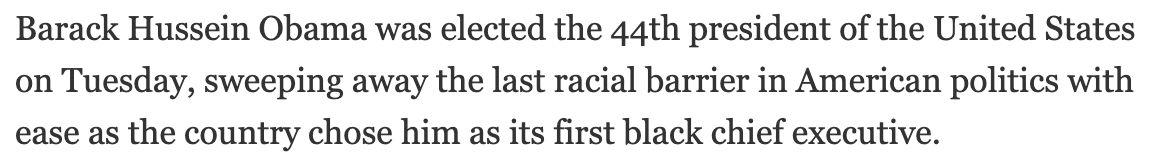
\includegraphics[scale=1.2]{obama-elected.png}
\end{center}
\vfill
\begin{itemize}
\item From this snippet, we can extract:
\begin{center}
\tt (United States, president, Barack Hussein Obama)
\end{center}
\item Why is this a hard problem?
\end{itemize}
\vfill

%%%%%%%%%%%%%%%%%%%%%%%%%%%%%%%%%%%%%%%%%%%%%%%%%%%%%%%%%%%%%%%%%%%%%%%%%%%%

\slide{Extracting Events}
\vfill
\begin{center}
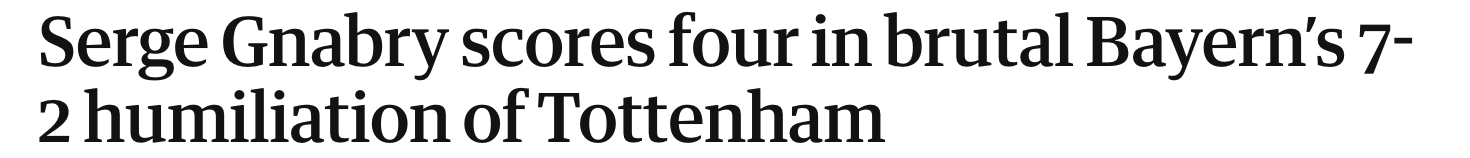
\includegraphics[scale=0.6]{tottenham-bayern1.png}
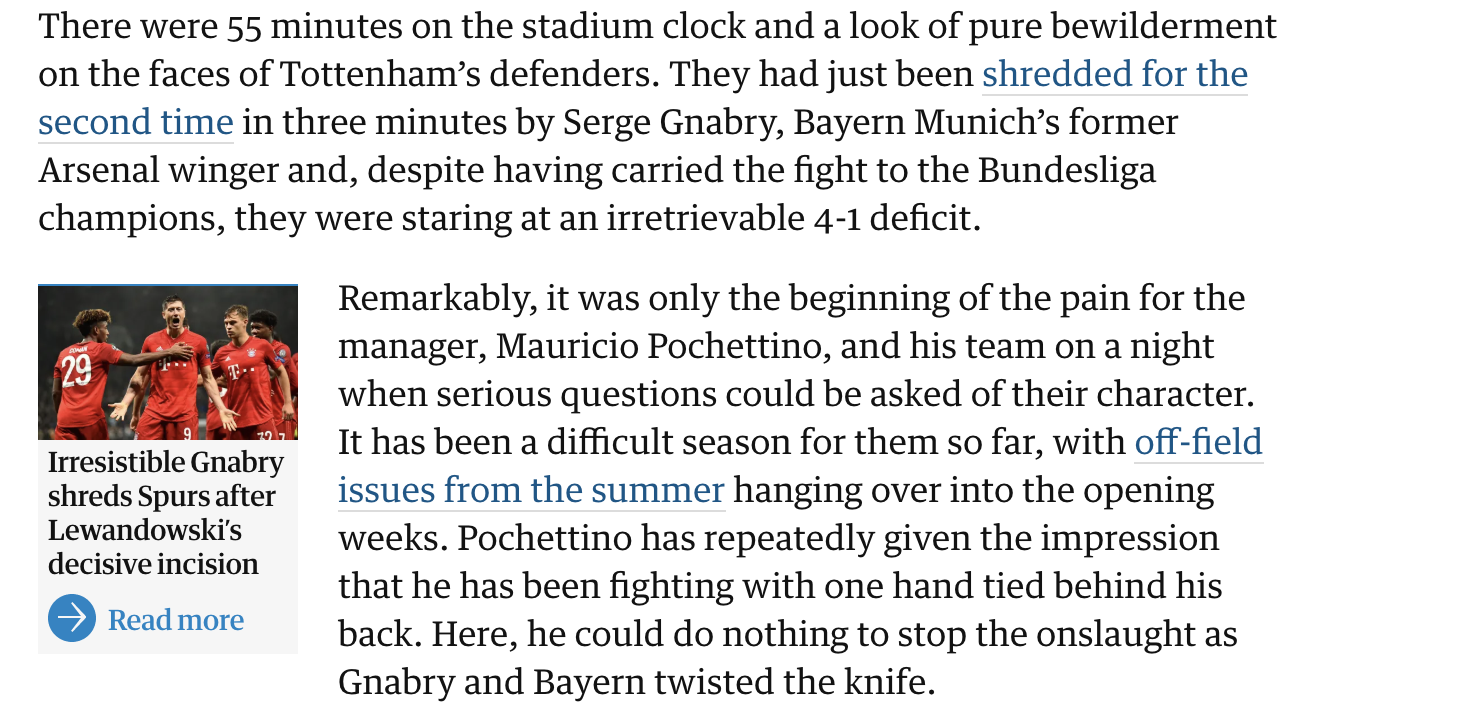
\includegraphics[scale=0.6]{tottenham-bayern2.png}
\end{center}
\begin{itemize}
\item Report of soccer game
\begin{itemize}
\item when? where? who? what? why? 
\item players involved, information about each player, each goal, audience size, ...?
\end{itemize}
\item Multiple data base tables, connection between entities
\end{itemize}
\vfill

%%%%%%%%%%%%%%%%%%%%%%%%%%%%%%%%%%%%%%%%%%%%%%%%%%%%%%%%%%%%%%%%%%%%%%%%%%%%

\slide{}
\vspace{85mm}
\begin{center}
{\huge structural knowledge}
\end{center}

%%%%%%%%%%%%%%%%%%%%%%%%%%%%%%%%%%%%%%%%%%%%

\slide{Ontologies}
\vfill
\begin{center}
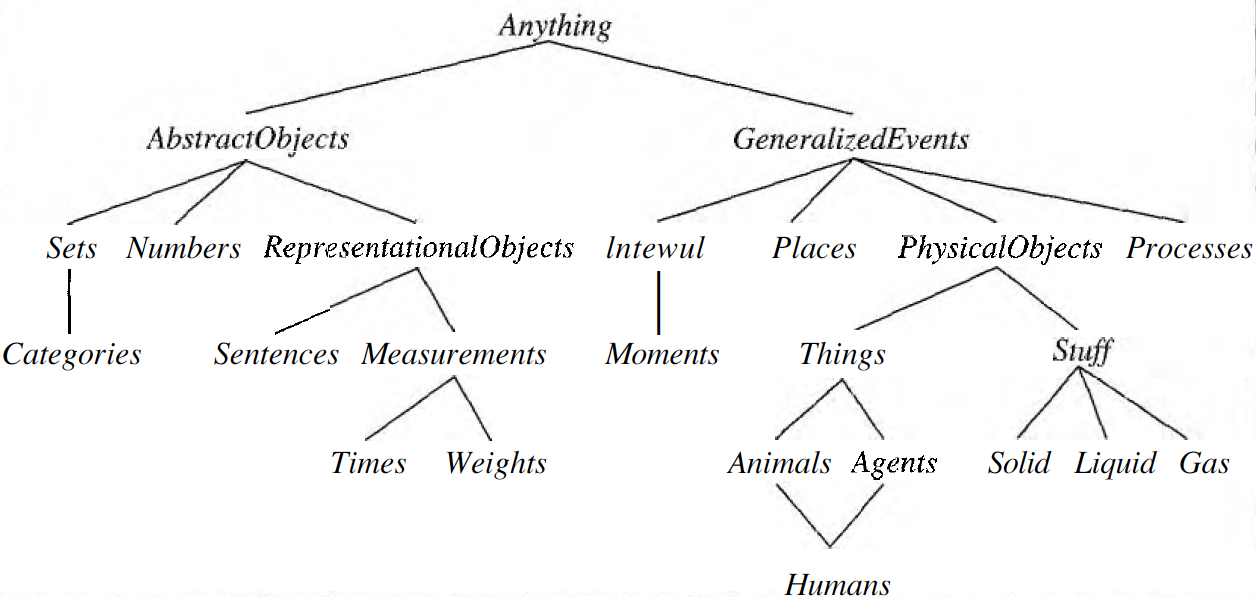
\includegraphics[width=24cm]{ontology.png}
\end{center}
\vfill

%%%%%%%%%%%%%%%%%%%%%%%%%%%%%%%%%%%%%%%%%%%%%%%%%%%%%%%%%%%%%%%%%%%%%%%%%%%%

\slide{Knowledge Graphs}
\vfill
\begin{center}
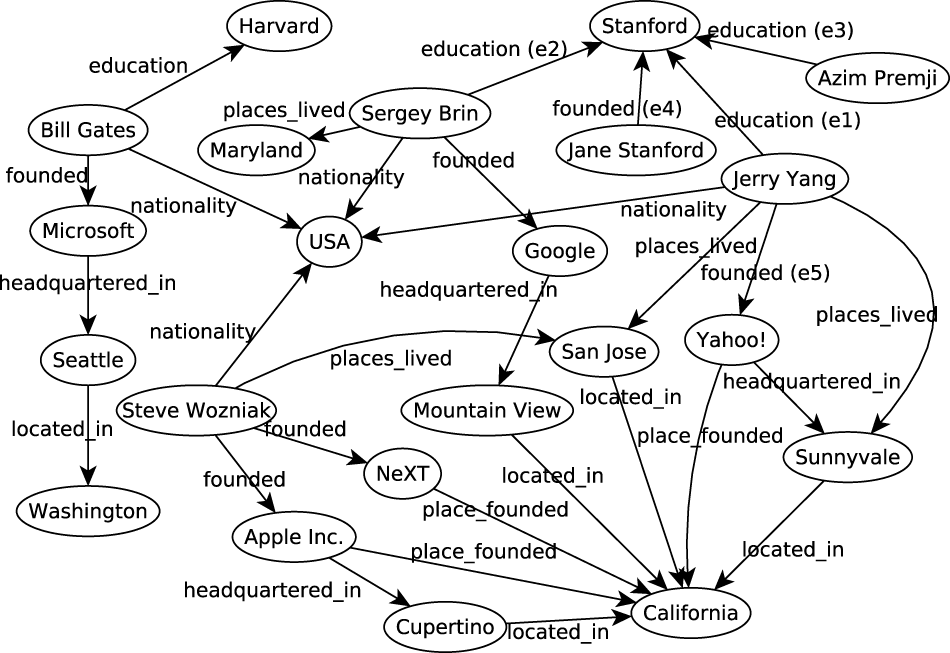
\includegraphics[width=21cm]{knowledge-graph.png}
\end{center}
\vfill

%%%%%%%%%%%%%%%%%%%%%%%%%%%%%%%%%%%%%%%%%%%%

\slide{Frames}
\vfill
\begin{center}
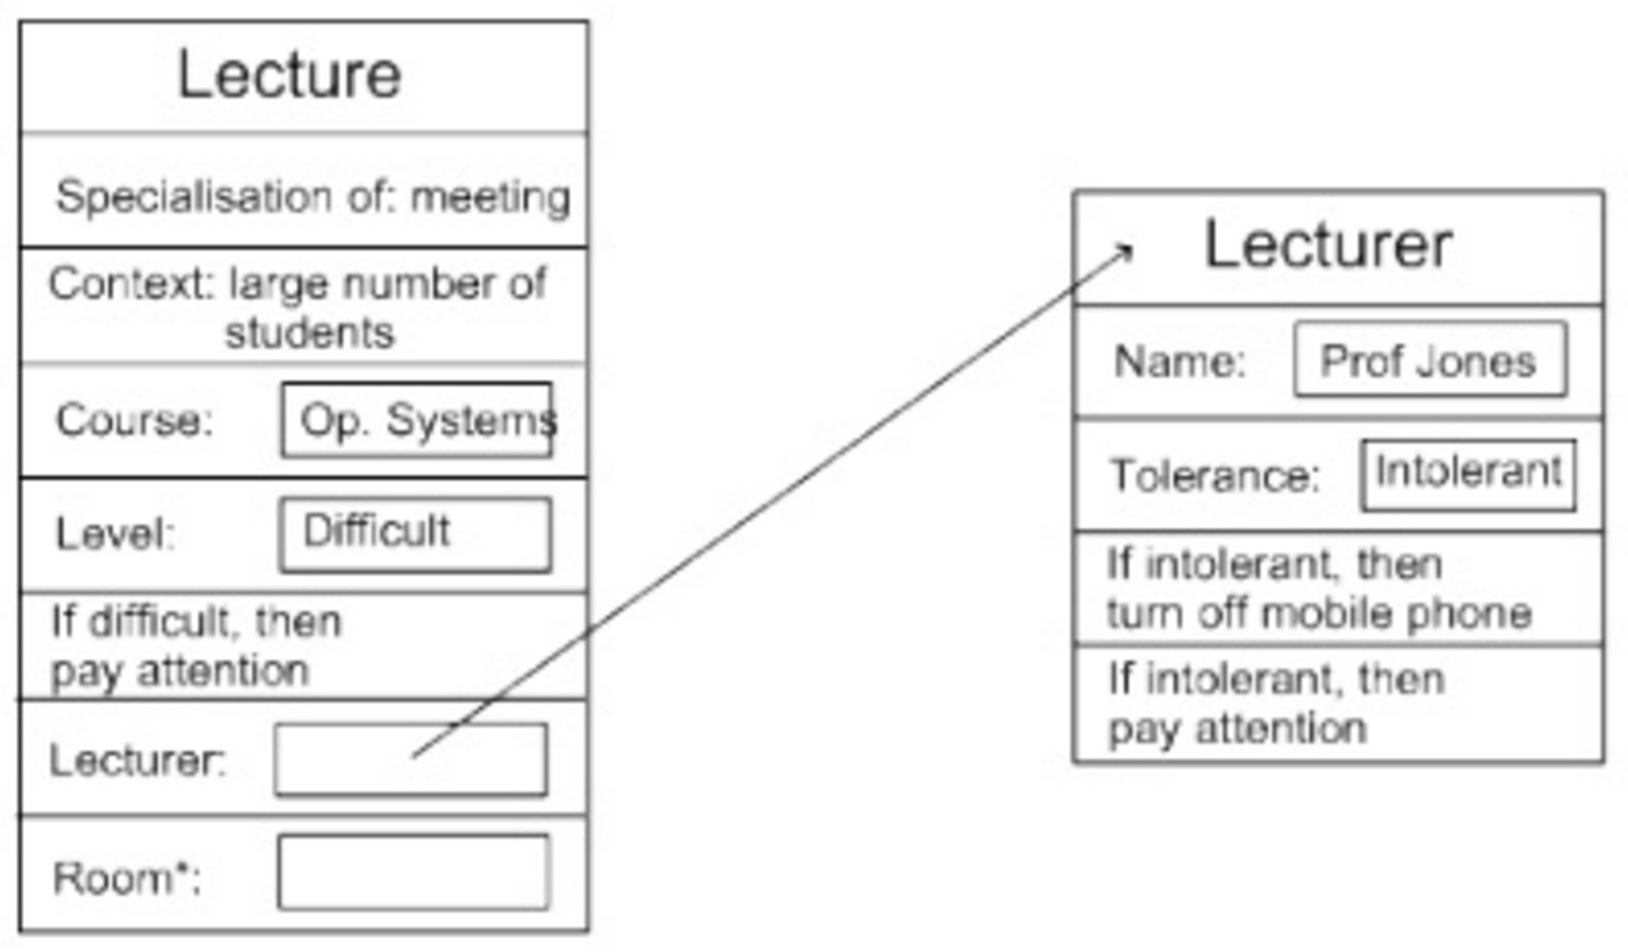
\includegraphics[width=24cm]{frame-example.png}
\end{center}
\vfill

%%%%%%%%%%%%%%%%%%%%%%%%%%%%%%%%%%%%%%%%%%%%

\slide{Scripts}
\vfill
\begin{center}
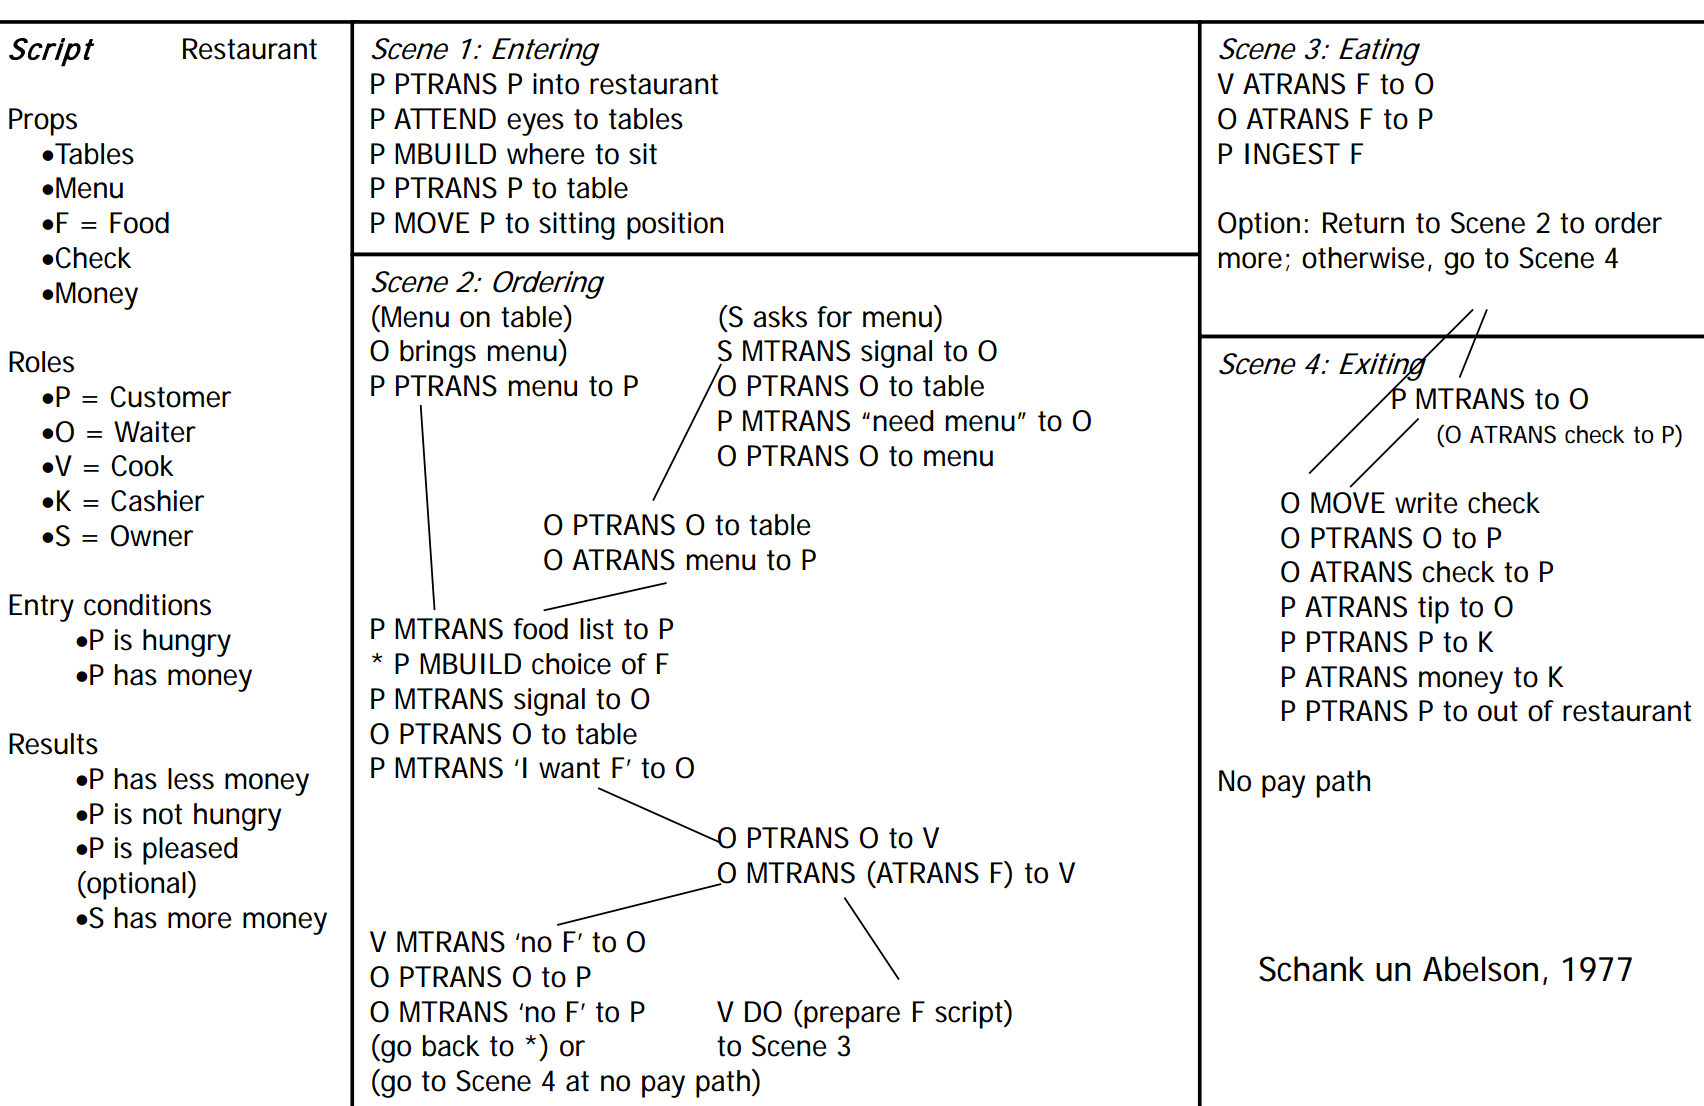
\includegraphics[width=23cm]{scripts-example-restaurant.png}
\end{center}
\vfill

%%%%%%%%%%%%%%%%%%%%%%%%%%%%%%%%%%%%%%%%%%%%%%%%%%%%%%%%%%%%%%%%%%%%%%%%%%%%

\slide{}
\vspace{85mm}
\begin{center}
{\huge named entities}
\end{center}

%%%%%%%%%%%%%%%%%%%%%%%%%%%%%%%%%%%%%%%%%%%%%%%%%%%%%%%%%%%%%%%%%%%%%%%%%%%%

\slide{Named Entities}
\vfill
\begin{itemize}
\item Essential processing step: identifying named entities
\item Types
\begin{itemize}
\item persons
\item geo-political entities (GPE)
\item events
\item dates
\item numbers
\end{itemize}
\end{itemize}
\vfill

%%%%%%%%%%%%%%%%%%%%%%%%%%%%%%%%%%%%%%%%%%%%%%%%%%%%%%%%%%%%%%%%%%%%%%%%%%%%

\slide{Example}
\vfill
\textcolor{darkgrey}{\begin{flushleft} \tt
\newcommand{\person}[1]{\textcolor{blue}{{\small [PERSON} #1{\small ]}}}
\newcommand{\gpe}[1]{\textcolor{purple}{{\small [GPE} #1{\small ]}}}
\newcommand{\nedate}[1]{\textcolor{brown}{{\small [DATE} #1{\small ]}}}
\newcommand{\event}[1]{\textcolor{verydarkgreen}{{\small [EVENT} #1{\small ]}}}
\newcommand{\nenumber}[1]{\textcolor{verydarkred}{{\small [NUMBER} #1{\small ]}}}
\person{Boris Johnson}'s \gpe{cabinet} is divided over how to proceed with \event{Brexit}, as the \person{prime minister} faces the stark choice of pressing ahead with his deal or gambling his premiership on a \nedate{pre-Christmas} general election. The \person{prime minister} told \person{MPs} at \nedate{Wednesday}'s \event{PMQs} that he was awaiting the decision of the \gpe{EU27} over whether to grant an extension before settling his next move. Some \person{cabinet ministers}, including the \person{\gpe{Northern Ireland} secretary, Julian Smith}, believe the majority of \nenumber{30} achieved by the \gpe{government} on the second reading of the \event{Brexit} bill on \nedate{Tuesday} suggests \person{Johnson}'s deal has enough support to carry it through all its stages in \gpe{parliament}.
\end{flushleft}}
% https://www.theguardian.com/politics/2019/oct/23/johnsons-cabinet-split-over-gambling-on-pre-christmas-election
\vfill

%%%%%%%%%%%%%%%%%%%%%%%%%%%%%%%%%%%%%%%%%%%%%%%%%%%%%%%%%%%%%%%%%%%%%%%%%%%%

\slide{Named Entity Tagging}
\vfill
\begin{itemize}
\item Problem broken up into two parts
\item Tagging where named entities start and end
\textcolor{darkgrey}{\begin{flushleft} \tt
\newcommand{\person}[1]{\textcolor{cyan}{{\small [NE} #1{\small ]}}}
\newcommand{\gpe}[1]{\textcolor{cyan}{{\small [NE} #1{\small ]}}}
\newcommand{\event}[1]{\textcolor{cyan}{{\small [NE} #1{\small ]}}}
\person{Boris Johnson}'s \gpe{cabinet} is divided over how to proceed with \event{Brexit}, as the \person{prime minister} faces the stark
\end{flushleft}}

\item Classification of types
\textcolor{darkgrey}{\begin{flushleft} \tt
\newcommand{\person}[1]{\textcolor{blue}{{\small [PERSON} #1{\small ]}}}
\newcommand{\gpe}[1]{\textcolor{purple}{{\small [GPE} #1{\small ]}}}
\newcommand{\event}[1]{\textcolor{verydarkgreen}{{\small [EVENT} #1{\small ]}}}
\person{Boris Johnson}'s \gpe{cabinet} is divided over how to proceed with \event{Brexit}, as the \person{prime minister} faces the stark 
\end{flushleft}}

\end{itemize}
\vfill


%%%%%%%%%%%%%%%%%%%%%%%%%%%%%%%%%%%%%%%%%%%%%%%%%%%%%%%%%%%%%%%%%%%%%%%%%%%%

\slide{Tagging}
\vfill
\begin{itemize}
\item Convert into BIO sequence (begin / intermediate / other)
\begin{center}
\tt \begin{tabular}{ll}
Boris & B\\
Johnson & I\\
's & O\\
cabinet & B\\
is & O\\
divided & O\\
over & O\\
how & O\\
to & O\\
proceed & O\\
with & O\\
Brexit & B\\
, & O
\end{tabular}
\end{center}
\end{itemize}
\vfill

%%%%%%%%%%%%%%%%%%%%%%%%%%%%%%%%%%%%%%%%%%%%%%%%%%%%%%%%%%%%%%%%%%%%%%%%%%%%

\slide{Bayes Rule}
\vfill
\begin{itemize}\itemsep 0mm
\item We want to find the best part-of-speech tag sequence \maths{$T$} for a sentence \maths{$S$}
\maths{\begin{equation*}
\mbox{argmax}_T\; p(T|S)\pause
\end{equation*}}
\item Bayes rule gives us
\maths{\begin{equation*}
p(T|S) = \frac{p(S|T)\;p(T)}{p(S)}\pause
\end{equation*}}
\item We can drop \maths{$p(S)$} if we are only interested in \maths{$\mbox{argmax}_T$}
\maths{\begin{equation*}
\mbox{argmax}_T \;p(T|S) = \mbox{argmax}_T \;p(S|T)\;p(T)
\end{equation*}}
\end{itemize}
\vfill

%%%%%%%%%%%%%%%%%%%%%%%%%%%%%%%%%%%%%%%%%%%%%%%%%%%%%%%%%%%%%%%%%%%%%%%%%%%%

\slide{Decomposing the Model}
\vfill
\begin{itemize}\itemsep 0mm
\item The mapping \maths{$p(S|T)$} can be decomposed into 
\maths{\begin{equation*}
p(S|T) = \prod_i p(w_i|t_i)\pause
\end{equation*}}
\item \maths{$p(T)$} could be called a {\em part-of-speech language model}, for which we can use an n-gram model:
\maths{\begin{equation*}
p(T) = p(t_1)\;p(t_2|t_1)\;p(t_3|t_1,t_2) ... p(t_n|t_{n-2},t_{n-1})\pause
\end{equation*}}
\item We can estimate \maths{$p(S|T)$} and \maths{$p(T)$} with maximum likelihood estimation (and maybe some smoothing)
\end{itemize}
\vfill

%%%%%%%%%%%%%%%%%%%%%%%%%%%%%%%%%%%%%%%%%%%%%%%%%%%%%%%%%%%%%%%%%%%%%%%%%%%%

\slide{Hidden Markov Model (HMM)}
\vfill
\begin{itemize}
\item The model we just developed is a {\bf Hidden Markov Model}
\item Elements of an HMM model:
\begin{itemize}
\item a set of states (here: the tags)
\item an output alphabet (here: words)
\item initial state (here: beginning of sentence)
\item state transition probabilities (here: \maths{$p(t_n|t_{n-2},t_{n-1})$})
\item symbol emission probabilities (here: \maths{$p(w_i|t_i)$})
\end{itemize}
\end{itemize}
\vfill

%%%%%%%%%%%%%%%%%%%%%%%%%%%%%%%%%%%%%%%%%%%%%%%%%%%%%%%%%%%%%%%%%%%%%%%%%%%%

\slide{Search for the Best Tag Sequence}
\vfill
\begin{itemize}
\item We have defined a model, but how do we use it?
\begin{itemize}
\item given: word sequence
\item wanted: tag sequence
\end{itemize}
\item If we consider a specific tag sequence, it is straight-forward to compute its probability
\maths{\begin{equation*}
p(S|T)\;p(T)=\prod_i p(w_i|t_i) \; p(t_i|t_{i-2},t_{i-1})
\end{equation*}}\vspace{-5mm}
\item Problem: if we have on average $c$ choices for each of the $n$ words, there are $c^n$ possible tag sequences, maybe too many to efficiently evaluate
\end{itemize}
\vfill

%%%%%%%%%%%%%%%%%%%%%%%%%%%%%%%%%%%%%%%%%%%%%%%%%%%%%%%%%%%%%%%%%%%%%%%%%%%%

\slide{Walking through the States}
\vfill
\begin{itemize}
\item First, we go to state {\em B} to emit {\tt Boris}:
\end{itemize}
\vfill
\begin{center}
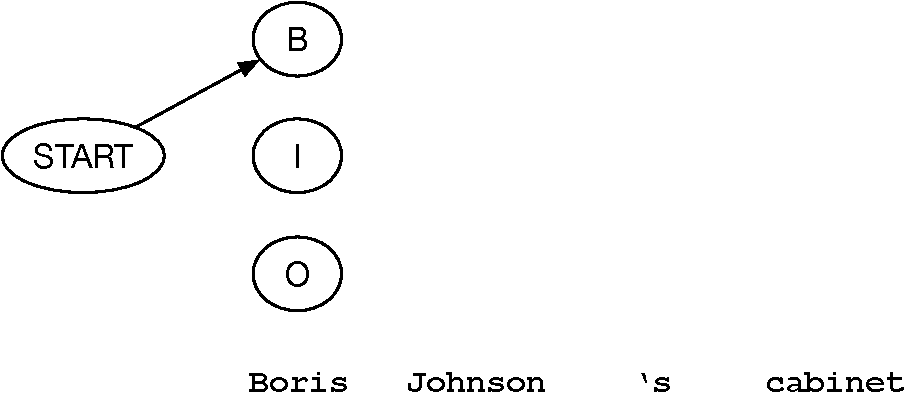
\includegraphics[scale=1.2]{hmm-search-ne1.pdf}
\end{center}
\vfill

%%%%%%%%%%%%%%%%%%%%%%%%%%%%%%%%%%%%%%%%%%%%%%%%%%%%%%%%%%%%%%%%%%%%%%%%%%%%


\slide{Walking through the States}
\vfill
\begin{itemize}
\item Then, we go to state {\em I} to emit {\tt Johnson}:
\end{itemize}
\vfill
\begin{center}
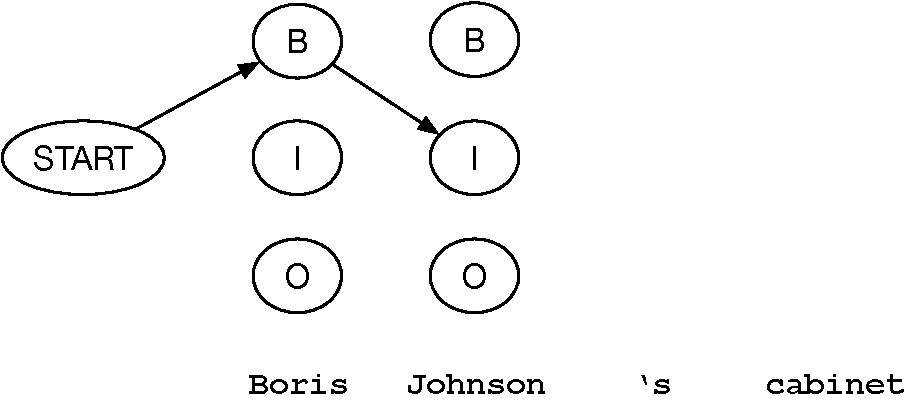
\includegraphics[scale=1.2]{hmm-search-ne2.pdf}
\end{center}
\vfill

%%%%%%%%%%%%%%%%%%%%%%%%%%%%%%%%%%%%%%%%%%%%%%%%%%%%%%%%%%%%%%%%%%%%%%%%%%%%


\slide{Walking through the States}
\vfill
\begin{itemize}
\item Of course, there are many possible paths:
\end{itemize}
\vfill
\begin{center}
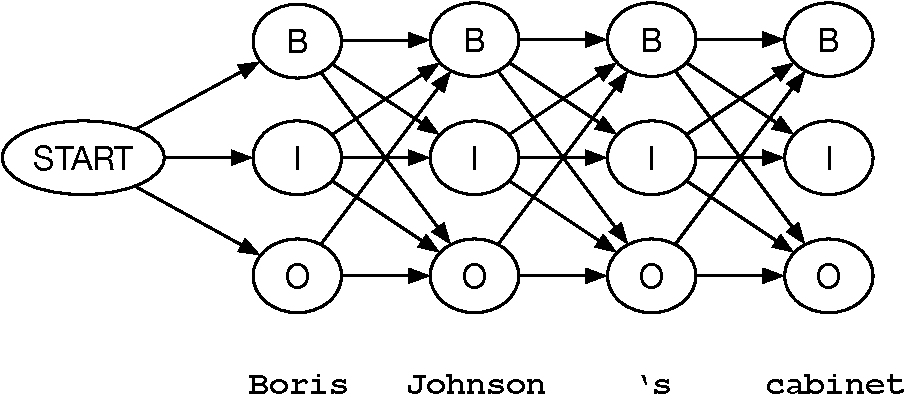
\includegraphics[scale=1.2]{hmm-search-ne3.pdf}
\end{center}
\vfill

%%%%%%%%%%%%%%%%%%%%%%%%%%%%%%%%%%%%%%%%%%%%%%%%%%%%%%%%%%%%%%%%%%%%%%%%%%%%

\slide{Viterbi Algorithm}
\vfill
\begin{itemize}
\item Intuition: Since state transition out of a state only depend on the current state (and not previous states), we can record for each state the optimal path\pause
\item We record:
\begin{itemize}
\item cheapest cost to state \maths{$j$} at step \maths{$s$} in \maths{$\delta_j(s)$}
\item backtrace from that state to best predecessor \maths{$\psi_j(s)$}\pause
\end{itemize}
\item Stepping through all states at each time steps allows us to compute
\begin{itemize}
\item \maths{$\delta_j(s+1) \; \; = \; \; \; \mbox{max}_{1 \le i \le N} \; \delta_i(s) \; p(t_i|t_j)\; p(w_s|t_j)$}
\item \maths{$\psi_j(s+1) = \mbox{argmax}_{1 \le i \le N} \; \delta_i(s) \; p(t_i|t_j)\; p(w_s|t_j)$}\pause
\end{itemize}
\item Best final state is \maths{$\mbox{argmax}_{1 \le i \le N} \; \delta_i(S+1)$}, we can backtrack from there
\end{itemize}
\vfill

%%%%%%%%%%%%%%%%%%%%%%%%%%%%%%%%%%%%%%%%%%%%%%%%%%%%%%%%%%%%%%%%%%%%%%%%%%%%

\slide{}
\vspace{85mm}
\begin{center}
{\huge entity linking}
\end{center}

%%%%%%%%%%%%%%%%%%%%%%%%%%%%%%%%%%%%%%%%%%%%%%%%%%%%%%%%%%%%%%%%%%%%%%%%%%%%

\slide{Same Person}
\vfill
\textcolor{darkgrey}{\begin{flushleft} \tt
\newcommand{\person}[1]{\textcolor{blue}{{\small [PERSON} #1{\small ]}}}
\newcommand{\gpe}[1]{#1}
\newcommand{\nedate}[1]{#1}
\newcommand{\event}[1]{#1}
\newcommand{\nenumber}[1]{#1}
\person{\textbf{Boris Johnson}}'s \gpe{cabinet} is divided over how to proceed with Brexit, as the \person{\textbf{prime minister}} faces the stark choice of pressing ahead with his deal or gambling his premiership on a \nedate{pre-Christmas} general election. The \person{\textbf{prime minister}} told MPs at \nedate{Wednesday}'s \event{PMQs} that he was awaiting the decision of the \gpe{EU27} over whether to grant an extension before settling his next move. Some cabinet ministers, including the secretary, Julian Smith, believe the majority of \nenumber{30} achieved by the \gpe{government} on the second reading of the \event{Brexit} bill on \nedate{Tuesday} suggests \person{\textbf{Johnson}}'s deal has enough support to carry it through all its stages in \gpe{parliament}.
\end{flushleft}}
\vfill
\begin{itemize}
\item Same person referred to 4 times in 3 different ways
\end{itemize}
\vfill

%%%%%%%%%%%%%%%%%%%%%%%%%%%%%%%%%%%%%%%%%%%%%%%%%%%%%%%%%%%%%%%%%%%%%%%%%%%%

\slide{Different Person, Same Name}
{\tiny
\begin{itemize}\itemsep 0mm
\item {\bf Explorers and Academics}
\begin{itemize}
\item John Smith (explorer) (1580--1631), helped found the Virginia Colony and became Colonial Governor of Virginia
\item John Smith (anatomist and chemist) (1721--1797), professor of anatomy and chemistry at the University of Oxford, 1766--97
\item John Smith (Cambridge, 1766), vice chancellor of the University of Cambridge, 1766 until 1767
\item John Smith (astronomer) (1711--1795), Lowndean Professor of Astronomy and Master of Caius
\item John Smith (lexicographer) (died 1809), professor of languages at Dartmouth College
\item John Smith (botanist) (1798--1888), curator of Kew Gardens
\item John Smith (physician) (c.1800--1879), Scottish physician specialising in treating the insane
\item John Smith (dentist) (1825--1910), founder of Edinburgh's School of Dentistry
\item John Smith (sociologist) (1927--2002), English sociologist
\end{itemize}
\item {\bf Arts}
\begin{itemize}
\item John Smith (engraver) (1652--1742), English mezzotint engraver
\item John Smith (English poet) (1662--1717), English poet and playwright
\item John Smith (clockmaker) (1770--1816), Scottish clockmaker
\item John Smith (architect) (1781--1852), Scottish architect
\item John Smith (art historian) (1781--1855), British art dealer
\item John Smith (Canadian poet) (born 1927), Canadian poet
\item John Smith (actor) (1931--1995), American actor
\item John Smith (English filmmaker) (born 1952), avant-garde filmmaker
\item John Smith (comics writer) (born 1967), British comics writer
\item John Smith (musician), English contemporary folk musician and recording artist
\end{itemize}
\item {\bf Politicians}
\begin{itemize}
\item John Smith (Victoria politician) (John Thomas Smith, 1816--1879), Australian politician
\item John Smith (New South Wales politician, born 1811) (1811--1895), Australian politician
\item John Smith (New South Wales politician, born 1821) (1821--1885), Scottish/Australian professor and politician
\item John Smith (Kent MPP), member of the 1st Ontario Legislative Assembly, 1867--1871
\item John Smith (Manitoba politician) (1817--1889), English-born farmer and politician in Manitoba
\item John Smith (Peel MPP) (1831--1909), Scottish-born Ontario businessman and political figure
\end{itemize}
\item ... many many more ...
\end{itemize}
}
\vfill

%%%%%%%%%%%%%%%%%%%%%%%%%%%%%%%%%%%%%%%%%%%%%%%%%%%%%%%%%%%%%%%%%%%%%%%%%%%%

\slide{Entity Linking}
\vfill
\begin{itemize}
\item Task: map a mention to an entity
\item Entity linking is often formulated as a ranking problem
\maths{\begin{equation*}
y^* = \text{argmax}_y \; \Psi(y, x, c) \hspace{3cm} y \in Y(x)\vspace{-5mm}
\end{equation*}}
where 
\begin{itemize}
\item \maths{$y$} is a target entity,
\item \maths{$x$} is a description of the mention
\item \maths{$Y(x)$} is a set of candidate entities
\item \maths{$c$} is a description of the context
\item \maths{$\Psi$} is a scoring function
\end{itemize}
\item Predefined name dictionary to restrict set of candidates $Y(x)$
\end{itemize}
\vfill

%%%%%%%%%%%%%%%%%%%%%%%%%%%%%%%%%%%%%%%%%%%%%%%%%%%%%%%%%%%%%%%%%%%%%%%%%%%%

\slide{Features}
\vfill
\begin{itemize}
\item Similarity of  mention string to  canonical entity name

\maths{$\Psi(\textcolor{darkgrey}{\tt ATLANTA}, \textcolor{darkgrey}{\tt Atlanta}, c) > 
\Psi(\textcolor{darkgrey}{\tt ATLANTA-HAWKS}, \textcolor{darkgrey}{\tt Atlanta}, c)$}

\item Popularity of the entity (e.g., measured by Wikipedia page views) 

\maths{$\Psi(\textcolor{darkgrey}{\tt ATLANTA, GEORGIA}, \textcolor{darkgrey}{\tt Atlanta}, c) > 
\Psi(\textcolor{darkgrey}{\tt ATLANTA, OHIO}, \textcolor{darkgrey}{\tt Atlanta}, c)$}

\item Entity type, as output by the named entity recognition system.

\maths{$\Psi(\textcolor{darkgrey}{\tt ATLANTA-CITY}, \textcolor{darkgrey}{\tt Atlanta}, c) > 
\Psi(\textcolor{darkgrey}{\tt ATLANTA-MAGAZINE}, \textcolor{darkgrey}{\tt Atlanta}, c)$}\\
 when tagged as LOCATION
\end{itemize}
\vfill

%%%%%%%%%%%%%%%%%%%%%%%%%%%%%%%%%%%%%%%%%%%%%%%%%%%%%%%%%%%%%%%%%%%%%%%%%%%%

\slide{}
\vspace{85mm}
\begin{center}
{\huge co-reference resolution}
\end{center}

%%%%%%%%%%%%%%%%%%%%%%%%%%%%%%%%%%%%%%%%%%%%%%%%%%%%%%%%%%%%%%%%%%%%%%%%%%%%

\slide{Pronomial Reference}
\vfill
\textcolor{darkgrey}{\begin{flushleft} \tt
\newcommand{\person}[1]{\textcolor{blue}{{\small [PERSON} #1{\small ]}}}
\newcommand{\pronoun}[1]{\textcolor{blue}{\textbf{#1}}}
\newcommand{\gpe}[1]{#1}
\newcommand{\nedate}[1]{#1}
\newcommand{\event}[1]{#1}
\newcommand{\nenumber}[1]{#1}
\person{\textbf{Boris Johnson}}'s \gpe{cabinet} is divided over how to proceed with \event{Brexit}, as the \person{\textbf{prime minister}} faces the stark choice of pressing ahead with \pronoun{his} deal or gambling \pronoun{his} premiership on a \nedate{pre-Christmas} general election. The \person{\textbf{prime minister}} told MPs at \nedate{Wednesday}'s \event{PMQs} that \pronoun{he} was awaiting the decision of the \gpe{EU27} over whether to grant an extension before settling \pronoun{his} next move. Some cabinet ministers, including the secretary, Julian Smith, believe the majority of \nenumber{30} achieved by the \gpe{government} on the second reading of the \event{Brexit} bill on \nedate{Tuesday} suggests \person{\textbf{Johnson}}'s deal has enough support to carry it through all its stages in \gpe{parliament}.
\end{flushleft}}
\vfill

%%%%%%%%%%%%%%%%%%%%%%%%%%%%%%%%%%%%%%%%%%%%%%%%%%%%%%%%%%%%%%%%%%%%%%%%%%%%

\slide{Some Terminology}
\vfill
\begin{description}
\item[Referring expression]
Part of  utterance used to identify or introduce an entity
\item[Referents]
are such entities (imagined to be) in the world
\item[Reference]
is the relation between a referring expression and a referent
\item[Coreference]
More than one referring expression is used to refer to the same entity
\item[Anaphora] Reference to, or depending on, a previously introduced entity
\end{description}
\vfill

%%%%%%%%%%%%%%%%%%%%%%%%%%%%%%%%%%%%%%%%%%%%%%%%%%%%%%%%%%%%%%%%%%%%%%%%%%%%

\slide{Coreference and Pronouns}
\vfill
\begin{itemize}
\item  Pronouns serve as anaphoric expressions when they rely on the previous discourse for their
interpretation
\begin{description}
\item[Definite pronouns]
\textcolor{darkgrey}{\tt He, she, it, they,} etc.
\item[Indefinite pronouns]
\textcolor{darkgrey}{\tt One, some, elsewhere, other,} etc.\pause
\end{description}
\item Some pronouns have other roles as well
\begin{itemize}
\item periphrastic it: \textcolor{darkgrey}{\tt It is raining}, \textcolor{darkgrey}{\tt It is surprising that you ate a banana}
\item generic they and one: \textcolor{darkgrey}{\tt They'll get you for that}, \textcolor{darkgrey}{\tt One doesn't do that sort of thing in
public}\pause
\end{itemize}
\item {\bf Antecedent}: expression from the previous discourse used in interpreting a pronoun
\end{itemize}
\vfill

%%%%%%%%%%%%%%%%%%%%%%%%%%%%%%%%%%%%%%%%%%%%%%%%%%%%%%%%%%%%%%%%%%%%%%%%%%%%

\slide{Reference Resolution}
\vfill
\begin{itemize}
\item Reference resolution is the process of determining the referent of a referring expression
\item Context obviously plays a crucial role in reference resolution
\begin{description}
\item[Situational]
The real-world surroundings (physical and temporal) for the discourse
\item[Mental]
The knowledge/beliefs of the participants
\item[Discourse]
What has been communicated so far\pause
\end{description}
\item Most approaches to implementing reference resolution distinguish two stages
\begin{enumerate}
\item Filter the set of possible referents by appeal to linguistic constraints
\item Rank the resulting candidates based on some set of heuristics
\end{enumerate}
\end{itemize}
\vfill

%%%%%%%%%%%%%%%%%%%%%%%%%%%%%%%%%%%%%%%%%%%%%%%%%%%%%%%%%%%%%%%%%%%%%%%%%%%%

\slide{Constraints on Pronouns: Feature Agreement}
\vfill
\begin{itemize}
\item English pronouns agree with number and/or gender of their antecedent
\textcolor{darkgrey}{\begin{flushleft} \tt \vspace{-5mm}
Robin has a new car. It/*She/*They is red.\\
Robin has a sister. *It/She/*They/*We is well-read.\\
Robin has three cars. *It/*She/They/*We are all red.\pause
\end{flushleft}}
\item As well as the person (but case is determined locally):
\textcolor{darkgrey}{\begin{flushleft} \tt \vspace{-5mm}
Robin and I were late. *Me/*They/We/I missed the show\\
Robin and I were late. The usher wouldn't let *we/*I/us/me in.\pause
\end{flushleft}}
\item German pronouns agree with number and gender of antecedent
\textcolor{darkgrey}{\begin{flushleft} \tt \vspace{-5mm}
Hier ist ein Apfel. Ich bedenke ob er/*sie/*es reif ist. [masc.]\\
Here's an apple. I wonder if *he/*she/it is ripe. [neuter]
\end{flushleft}}
\end{itemize}
\vfill

%%%%%%%%%%%%%%%%%%%%%%%%%%%%%%%%%%%%%%%%%%%%%%%%%%%%%%%%%%%%%%%%%%%%%%%%%%%%

\slide{Constraints on Pronouns: Syntax}
\vfill
\begin{itemize}
\item When the text is in the same sentence, pronominal coreference is subject to binding
conditions
\textcolor{darkgrey}{\begin{flushleft} \tt \vspace{-5mm}
Joe likes him \textcolor{black}{\rm vs.} John likes himself\\[3mm]
Joe thinks Ann likes him/herself\\
\textcolor{black}{\rm vs.} *Joe thinks Ann likes himself\\[3mm]
Her brother admires Ann \textcolor{black}{\rm Whose brother?}\pause
\end{flushleft}}
\item And, sometimes, to selectional restrictions based on the verb that governs it
\textcolor{darkgrey}{\begin{flushleft} \tt \vspace{-5mm}
Joe parks his car in the garage. He has driven it around for hours
\end{flushleft}}\vspace{-7mm}
\textcolor{darkgrey}{it} = \textcolor{darkgrey}{the car}, \textcolor{darkgrey}{it} $\neq$ \textcolor{darkgrey}{garage}
\textcolor{darkgrey}{\begin{flushleft} \tt \vspace{0mm}
I picked up the book and sat in a chair. It broke
\end{flushleft}}\vspace{-7mm}
\textcolor{darkgrey}{it} = \textcolor{darkgrey}{chair}, \textcolor{darkgrey}{it} $\neq$ \textcolor{darkgrey}{book}
\end{itemize}
\vfill

%%%%%%%%%%%%%%%%%%%%%%%%%%%%%%%%%%%%%%%%%%%%%%%%%%%%%%%%%%%%%%%%%%%%%%%%%%%%

\slide{Constraints Not Enough}
\vfill
\begin{itemize}
\item  The kind of strong constraints we've just seen are not always enough to reduce the candidate
set for resolution to a single entity
\textcolor{darkgrey}{\begin{flushleft} \tt
John punched Bill. He broke his jaw\\
John punched Bill. He broke his hand\\[1cm]
Tom hates her husband, but Jane worked for him anyway\\
Tom hates her husband, but Jane stays with him anyway
\end{flushleft}}
\end{itemize}
\vfill

%%%%%%%%%%%%%%%%%%%%%%%%%%%%%%%%%%%%%%%%%%%%%%%%%%%%%%%%%%%%%%%%%%%%%%%%%%%%

\slide{Heuristics for Pronoun Interpretation}
\vfill
\begin{itemize}
\item Many different features influence how a listener will resolve a definite pronoun (i.e., what they
will take to be its antecedent)
\end{itemize}
\begin{description}
\item[Recency]
The most recently introduced entity is a better candidate
\textcolor{darkgrey}{\begin{flushleft} \tt
 First Robin bought a phone, and then a tablet. Kim is always borrowing it\pause
\end{flushleft}}
\item[Grammatical role]
Some grammatical roles (e.g. SUBJECT) are felt to be more salient than others (e.g.,
OBJECT)
\textcolor{darkgrey}{\begin{flushleft} \tt
Bill went to the pub with John. He bought the first round
\end{flushleft}}
\textcolor{darkgrey}{\tt John} is more recent, but \textcolor{darkgrey}{\tt Bill} is more salient.
\end{description}
\vfill

%%%%%%%%%%%%%%%%%%%%%%%%%%%%%%%%%%%%%%%%%%%%%%%%%%%%%%%%%%%%%%%%%%%%%%%%%%%%

\slide{Heuristics}
\vfill
\begin{description}
\item[Repeated mention]
A repeatedly-mentioned entity is likely to be mentioned again
\textcolor{darkgrey}{\begin{flushleft} \tt
John needed portable web access for his new job. He decided he wanted
something classy. Bill went to the Apple store with him. He bought an
iPad.
\end{flushleft}}
\textcolor{darkgrey}{\tt Bill} is the previous subject, but \textcolor{darkgrey}{\tt John}'s repeated mentions tips the balance.\pause
\item[Parallelism]
Parallel syntactic constructs can create an expectation of coreference in parallel positions
\textcolor{darkgrey}{\begin{flushleft} \tt
Susan went with Ann to the cinema. Carol went with her to the pub
\end{flushleft}}
\end{description}
\vfill

%%%%%%%%%%%%%%%%%%%%%%%%%%%%%%%%%%%%%%%%%%%%%%%%%%%%%%%%%%%%%%%%%%%%%%%%%%%%

\slide{Heuristics}
\vfill
\begin{description}
\item[Verb semantics]
A verb may serve to foreground one of its argument positions for subsequent reference
because of its semantics
\textcolor{darkgrey}{\begin{flushleft} \tt
John criticized Bill after he broke his promise vs. John telephoned Bill after
he broke his promise\\[3mm]
Louise apologized to/praised Sandra because she ...\pause
\end{flushleft}}
\item[World knowledge]
At the end of the day, sometimes only one reading makes sense
\textcolor{darkgrey}{\begin{flushleft} \tt
The city council denied the demonstrators a permit because they feared violence
\end{flushleft}}
vs. 
\textcolor{darkgrey}{\begin{flushleft} \tt
The city council denied the demonstrators a permit because they advocated
violence
\end{flushleft}}
\end{description}
\vfill

%%%%%%%%%%%%%%%%%%%%%%%%%%%%%%%%%%%%%%%%%%%%%%%%%%%%%%%%%%%%%%%%%%%%%%%%%%%%

\slide{Automatic Methods}
\vfill
\begin{itemize}
\item Rich history of automatic definite reference and pronoun resolution systems
\begin{itemize}
\item initially rule-based
\item more recently using machine learning
\end{itemize}
\item Viewed as a simple binomial classification task
\begin{itemize}
\item for every pair of referring expressions
\item are they coreferential, or not?
\end{itemize}
\end{itemize}
\vfill

%%%%%%%%%%%%%%%%%%%%%%%%%%%%%%%%%%%%%%%%%%%%%%%%%%%%%%%%%%%%%%%%%%%%%%%%%%%%

\slide{Supervised Training}
\vfill
\begin{itemize}
\item Given an corpus annotated for coreference, to train a model we simply
\begin{itemize}
\item given an NP$_k$ that is known to co-refer with NP$_j$ where NP$_j$ is the closest such NP, create
a positive training instance (NP$_k$, NP$_j$).
\item for all NPs between NP$_k$ and NP$_j$, create a negative training instance(NP$_k$, NP$_{j+1}$),
(NP$_k$, NP$_{j+2}$), etc.\pause
\end{itemize}
\item Tabulate the value of likely candidate features,\pause such as
\begin{itemize}
\item the nature of NP$_k$ and NP$_j$: pronouns, definite NPs, demonstrative NPs (this/that/these/
those X), proper names;\pause
\item distance betwen NP$_k$ and NP$_j$: 0 if same sentence, 1 if adjacent sentence, etc.;\pause
\item whether NP$_k$ and NP$_j$ agree in number;\pause
\item whether NP$_k$ and NP$_j$ agree in gender;\pause
\item whether their semantic classes are in agreement;\pause
\item edit distance between NP$_k$ and NP$_j$;
\end{itemize}
\item Use any supervised learning method to train a model
\end{itemize}
\vfill

%%%%%%%%%%%%%%%%%%%%%%%%%%%%%%%%%%%%%%%%%%%%%%%%%%%%%%%%%%%%%%%%%%%%%%%%%%%%

\slide{}
\vspace{85mm}
\begin{center}
{\huge relation extraction}
\end{center}

%%%%%%%%%%%%%%%%%%%%%%%%%%%%%%%%%%%%%%%%%%%%%%%%%%%%%%%%%%%%%%%%%%%%%%%%%%%%

\slide{Relations}
\vfill
\begin{itemize}\itemsep 1cm
\item We may be interested in relations of a specific type
\item Example: birthplaces
\textcolor{darkgrey}{\begin{flushleft} \tt
Bill Clinton was born in the small town of Hope, Arkansas, ...
George Walker Bush was born in New Haven, Connecticut, while ...\\
Obama was born in Hawaii, studied at Columbia and Harvard, ...\\
\end{flushleft}}
\item Broad category: {\small ENTITY-ORIGIN}
\end{itemize}
\vfill

%%%%%%%%%%%%%%%%%%%%%%%%%%%%%%%%%%%%%%%%%%%%%%%%%%%%%%%%%%%%%%%%%%%%%%%%%%%%

\slide{Types of Relations}
\vfill
\begin{itemize}
\item Types of relations from SemEval-2010
\end{itemize}
\vfill
\begin{tabular}{ll}
\small CAUSE-EFFECT & \example{those cancers were caused by radiation exposures} \\
\small INSTRUMENT-AGENCY & \example{phone operator} \\
\small PRODUCT-PRODUCER & \example{a factory manufactures suits} \\
\small CONTENT-CONTAINER & \example{a bottle of honey was weighed} \\
\small ENTITY-ORIGIN & \example{letters from foreign countries} \\
\small ENTITY-DESTINATION & \example{the boy went to bed} \\
\small COMPONENT-WHOLE & \example{my apartment has a large kitchen}  \\
\small MEMBER-COLLECTION & \example{there are many trees in the forest}  \\
\small COMMUNICATION-TOPIC & \example{the lecture was about semantics}  \\
\end{tabular}
\vfill

%%%%%%%%%%%%%%%%%%%%%%%%%%%%%%%%%%%%%%%%%%%%%%%%%%%%%%%%%%%%%%%%%%%%%%%%%%%%

\slide{Pattern-Based Relation Extraction}
\vfill
\begin{itemize}
\item Surface patterns
\textcolor{darkgrey}{\begin{flushleft} \tt
[PERSON] was born in [LOCATION]\\
\end{flushleft}}
\item Not robust to small variations
\textcolor{darkgrey}{\begin{flushleft} \tt
Bill Clinton was born in \textcolor{darkred}{the small town of} Hope, Arkansas, ...\\
Ronald Reagan \textcolor{darkred}{who} was born in Tampico, Illinois ...\\
Jimmy Carter was born \textcolor{darkred}{October 1, 1924} in Plains, GA.
\end{flushleft}}
\item Possibly many patterns needed
\begin{itemize}
\item hand-crafted patterns likely high precision, low recall
\item learned patterns require annotated training data or known examples
\end{itemize}
\end{itemize}
\vfill

%%%%%%%%%%%%%%%%%%%%%%%%%%%%%%%%%%%%%%%%%%%%%%%%%%%%%%%%%%%%%%%%%%%%%%%%%%%%

\slide{Syntactic Patterns}
\vfill
\begin{itemize}\itemsep 1cm
\item Patterns can be also defined over the syntactic relations
\item Dependency relationships
\textcolor{darkgrey}{\begin{flushleft} \tt
[PERSON] $\leftarrow$SUBJ{\rm ---} born {\rm ---}PP-LOC$\rightarrow$ [LOCATION]
\end{flushleft}}
\item Recall: semantic roles
\end{itemize}
\vfill

%%%%%%%%%%%%%%%%%%%%%%%%%%%%%%%%%%%%%%%%%%%%%%%%%%%%%%%%%%%%%%%%%%%%%%%%%%%%

\slide{Learning Patterns}
\vfill
\begin{itemize}
\item Given a set of examples for a relation \textcolor{darkgrey}{\tt {\small ENTITY-ORIGIN}(person, location)}
\item Automatically label text where both \textcolor{darkgrey}{\tt person} and \textcolor{darkgrey}{\tt location} occur
\item Use this as training data to learn classifier
\item Features
\begin{itemize}
\item properties of the entities
\item words and n-gram between and around entities
\item syntactic dependency path between entities
\end{itemize}
\end{itemize}
\vfill

%%%%%%%%%%%%%%%%%%%%%%%%%%%%%%%%%%%%%%%%%%%%%%%%%%%%%%%%%%%%%%%%%%%%%%%%%%%%

\slide{}
\vspace{85mm}
\begin{center}
{\huge knowledge base population}
\end{center}

%%%%%%%%%%%%%%%%%%%%%%%%%%%%%%%%%%%%%%%%%%%%%%%%%%%%%%%%%%%%%%%%%%%%%%%%%%%%

\slide{Wikipedia Infobox}
\vspace{-2cm}
\begin{flushright}
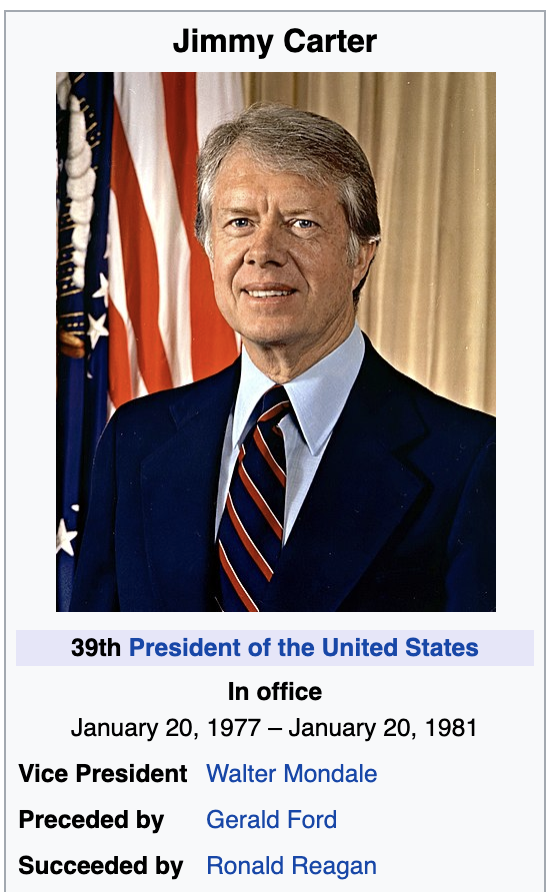
\includegraphics[scale=0.65]{jimmy-carter1.png}\\
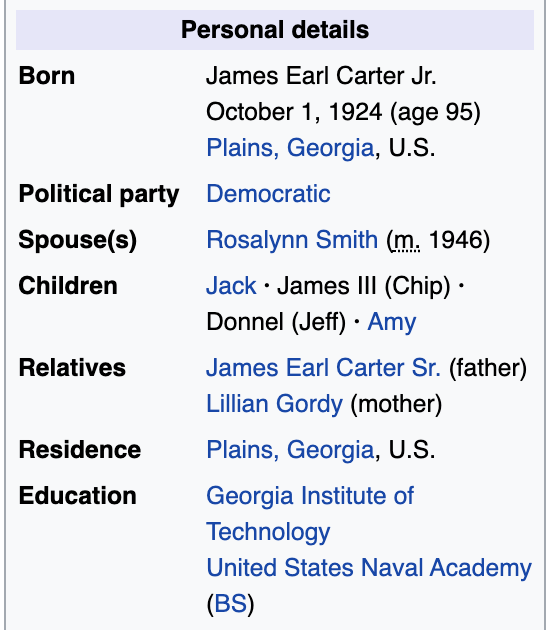
\includegraphics[scale=0.65]{jimmy-carter2.png}
\end{flushright}\vspace{-13cm}
\begin{itemize}
\item Given a frame
\item Slot filling
\item Each slot a relation
\item Possibly multiple entries in a slot\\
(children, education)
\end{itemize}

%%%%%%%%%%%%%%%%%%%%%%%%%%%%%%%%%%%%%%%%%%%%%%%%%%%%%%%%%%%%%%%%%%%%%%%%%%%%

\slide{Information Fusion}
\vfill
\begin{center}
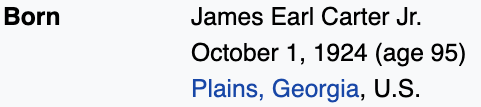
\includegraphics[scale=1.8]{jimmy-carter2a.png}
\end{center}
\vfill
\begin{itemize}
\item Combine information from multiple text sources
\end{itemize}\vspace{5mm}
\textcolor{darkgrey}{\begin{flushleft}\tt
Jimmy Carter celebrates his birthday today on October 1.\\
Born in 1924, Carter is the oldest president alive, ...\\
President Carter who hails from Plains, Georga, ...
\end{flushleft}}
\vfill

%%%%%%%%%%%%%%%%%%%%%%%%%%%%%%%%%%%%%%%%%%%%%%%%%%%%%%%%%%%%%%%%%%%%%%%%%%%%

\slide{Events}
\vfill
\begin{itemize}
\item Events involve multiple relations
\item Limited to a specific time frame
\item Event co-reference
\begin{itemize}
\item multiple mentions of same event
\item mention same time frame, same actors, etc.
\item clustering? linking?
\end{itemize}
\item Relations between events
\begin{itemize}
\item temporal relationships
\item causal relationships
\end{itemize}
\end{itemize}
\vfill

%%%%%%%%%%%%%%%%%%%%%%%%%%%%%%%%%%%%%%%%%%%%%%%%%%%%%%%%%%%%%%%%%%%%%%%%%%%%

\slide{Hedges, Denials, Hypothetical}
\vfill
\begin{itemize}\itemsep 2mm
\item Examples
\textcolor{darkgrey}{\begin{enumerate}\itemsep 0mm \tt
\item GM will lay off workers.
\item A spokesman for GM said GM will lay off workers.
\item GM may lay off workers.
\item The politician claimed that GM will lay off workers. 
\item Some wish GM would lay off workers.
\item Will GM lay off workers?
\item Many wonder whether GM will lay off workers.
\item This suggests that GM will lay off workers.
\end{enumerate}}
\item Probability of proposition (\textcolor{darkgrey}{\tt may})
\item Hedging (\textcolor{darkgrey}{\tt suggests})
\item Attribution (\textcolor{darkgrey}{\tt spokesman said}, \textcolor{darkgrey}{\tt politician claimed})
\end{itemize}
\vfill

%%%%%%%%%%%%%%%%%%%%%%%%%%%%%%%%%%%%%%%%%%%%%%%%%%%%%%%%%%%%%%%%%%%%%%%%%%%%

\slide{}
\vspace{85mm}
\begin{center}
{\huge questions?}
\end{center}

%%%%%%%%%%%%%%%%%%%%%%%%%%%%%%%%%%%%%%%%%%%%%%%%%%%%%%%%%%%%%%%%%%%%%%%%%%%%


\end{document}
